%===============================================================================
% LaTeX sjabloon voor de bachelorproef toegepaste informatica aan HOGENT
% Meer info op https://github.com/HoGentTIN/latex-hogent-report
%===============================================================================

\documentclass[dutch,dit,thesis]{hogentreport}

% TODO:
% - If necessary, replace the option `dit`' with your own department!
%   Valid entries are dbo, dbt, dgz, dit, dlo, dog, dsa, soa
% - If you write your thesis in English (remark: only possible after getting
%   explicit approval!), remove the option "dutch," or replace with "english".

\usepackage{lipsum} % For blind text, can be removed after adding actual content

%% Pictures to include in the text can be put in the graphics/ folder
\graphicspath{{graphics/}}

%% For source code highlighting, requires pygments to be installed
%% Compile with the -shell-escape flag!
\usepackage[section]{minted}
\usemintedstyle{solarized-light}
\definecolor{bg}{RGB}{253,246,227} %% Set the background color of the codeframe

%% Change this line to edit the line numbering style:
\renewcommand{\theFancyVerbLine}{\ttfamily\scriptsize\arabic{FancyVerbLine}}

%% Macro definition to load external java source files with \javacode{filename}:
\newmintedfile[javacode]{java}{
    bgcolor=bg,
    fontfamily=tt,
    linenos=true,
    numberblanklines=true,
    numbersep=5pt,
    gobble=0,
    framesep=2mm,
    funcnamehighlighting=true,
    tabsize=4,
    obeytabs=false,
    breaklines=true,
    mathescape=false
    samepage=false,
    showspaces=false,
    showtabs =false,
    texcl=false,
}

% Other packages not already included can be imported here

%%---------- Document metadata -------------------------------------------------
% TODO: Replace this with your own information
\author{Ernst Aarden}
\supervisor{Dhr. F. Van Houte}
\cosupervisor{Mevr. S. Beeckman}
\title[Optionele ondertitel]%
    {Titel van de bachelorproef}
\academicyear{\advance\year by -1 \the\year--\advance\year by 1 \the\year}
\examperiod{1}
\degreesought{\IfLanguageName{dutch}{Professionele bachelor in de toegepaste informatica}{Bachelor of applied computer science}}
\partialthesis{false} %% To display 'in partial fulfilment'
%\institution{Internshipcompany BVBA.}

%% Add global exceptions to the hyphenation here
\hyphenation{back-slash}

%% The bibliography (style and settings are  found in hogentthesis.cls)
\addbibresource{bachproef.bib}            %% Bibliography file
\addbibresource{../voorstel/voorstel.bib} %% Bibliography research proposal
\defbibheading{bibempty}{}

%% Prevent empty pages for right-handed chapter starts in twoside mode
\renewcommand{\cleardoublepage}{\clearpage}

\renewcommand{\arraystretch}{1.2}

%% Content starts here.
\begin{document}

%---------- Front matter -------------------------------------------------------

\frontmatter

\hypersetup{pageanchor=false} %% Disable page numbering references
%% Render a Dutch outer title page if the main language is English
\IfLanguageName{english}{%
    %% If necessary, information can be changed here
    \degreesought{Professionele Bachelor toegepaste informatica}%
    \begin{otherlanguage}{dutch}%
       \maketitle%
    \end{otherlanguage}%
}{}

%% Generates title page content
\maketitle
\hypersetup{pageanchor=true}

%%=============================================================================
%% Voorwoord
%%=============================================================================

\chapter*{\IfLanguageName{dutch}{Woord vooraf}{Preface}}%
\label{ch:voorwoord}

%% TODO:
%% Het voorwoord is het enige deel van de bachelorproef waar je vanuit je
%% eigen standpunt (``ik-vorm'') mag schrijven. Je kan hier bv. motiveren
%% waarom jij het onderwerp wil bespreken.
%% Vergeet ook niet te bedanken wie je geholpen/gesteund/... heeft

%%=============================================================================
%% Samenvatting
%%=============================================================================

% TODO: De "abstract" of samenvatting is een kernachtige (~ 1 blz. voor een
% thesis) synthese van het document.
%
% Een goede abstract biedt een kernachtig antwoord op volgende vragen:
%
% 1. Waarover gaat de bachelorproef?
% 2. Waarom heb je er over geschreven?
% 3. Hoe heb je het onderzoek uitgevoerd?
% 4. Wat waren de resultaten? Wat blijkt uit je onderzoek?
% 5. Wat betekenen je resultaten? Wat is de relevantie voor het werkveld?
%
% Daarom bestaat een abstract uit volgende componenten:
%
% - inleiding + kaderen thema
% - probleemstelling
% - (centrale) onderzoeksvraag
% - onderzoeksdoelstelling
% - methodologie
% - resultaten (beperk tot de belangrijkste, relevant voor de onderzoeksvraag)
% - conclusies, aanbevelingen, beperkingen
%
% LET OP! Een samenvatting is GEEN voorwoord!

%%---------- Nederlandse samenvatting -----------------------------------------
%
% TODO: Als je je bachelorproef in het Engels schrijft, moet je eerst een
% Nederlandse samenvatting invoegen. Haal daarvoor onderstaande code uit
% commentaar.
% Wie zijn bachelorproef in het Nederlands schrijft, kan dit negeren, de inhoud
% wordt niet in het document ingevoegd.

\IfLanguageName{english}{%
\selectlanguage{dutch}
\chapter*{Samenvatting}
\lipsum[1-4]
\selectlanguage{english}
}{}

%%---------- Samenvatting -----------------------------------------------------
% De samenvatting in de hoofdtaal van het document

\chapter*{\IfLanguageName{dutch}{Samenvatting}{Abstract}}

\lipsum[1-4]


%---------- Inhoud, lijst figuren, ... -----------------------------------------

\tableofcontents

% In a list of figures, the complete caption will be included. To prevent this,
% ALWAYS add a short description in the caption!
%
%  \caption[short description]{elaborate description}
%
% If you do, only the short description will be used in the list of figures

\listoffigures

% If you included tables and/or source code listings, uncomment the appropriate
% lines.
%\listoftables
%\listoflistings

% Als je een lijst van afkortingen of termen wil toevoegen, dan hoort die
% hier thuis. Gebruik bijvoorbeeld de ``glossaries'' package.
% https://www.overleaf.com/learn/latex/Glossaries

%---------- Kern ---------------------------------------------------------------

\mainmatter{}

% De eerste hoofdstukken van een bachelorproef zijn meestal een inleiding op
% het onderwerp, literatuurstudie en verantwoording methodologie.
% Aarzel niet om een meer beschrijvende titel aan deze hoofdstukken te geven of
% om bijvoorbeeld de inleiding en/of stand van zaken over meerdere hoofdstukken
% te verspreiden!

%%=============================================================================
%% Inleiding
%%=============================================================================

\chapter{\IfLanguageName{dutch}{Inleiding}{Introduction}}%
\label{ch:inleiding}

De inleiding moet de lezer net genoeg informatie verschaffen om het onderwerp te begrijpen en in te zien waarom de onderzoeksvraag de moeite waard is om te onderzoeken. In de inleiding ga je literatuurverwijzingen beperken, zodat de tekst vlot leesbaar blijft. Je kan de inleiding verder onderverdelen in secties als dit de tekst verduidelijkt. Zaken die aan bod kunnen komen in de inleiding~\autocite{Pollefliet2011}:

\begin{itemize}
  \item context, achtergrond
  \item afbakenen van het onderwerp
  \item verantwoording van het onderwerp, methodologie
  \item probleemstelling
  \item onderzoeksdoelstelling
  \item onderzoeksvraag
  \item \ldots
\end{itemize}

\section{\IfLanguageName{dutch}{Probleemstelling}{Problem Statement}}%
\label{sec:probleemstelling}

Uit je probleemstelling moet duidelijk zijn dat je onderzoek een meerwaarde heeft voor een concrete doelgroep. De doelgroep moet goed gedefinieerd en afgelijnd zijn. Doelgroepen als ``bedrijven,'' ``KMO's'', systeembeheerders, enz.~zijn nog te vaag. Als je een lijstje kan maken van de personen/organisaties die een meerwaarde zullen vinden in deze bachelorproef (dit is eigenlijk je steekproefkader), dan is dat een indicatie dat de doelgroep goed gedefinieerd is. Dit kan een enkel bedrijf zijn of zelfs één persoon (je co-promotor/opdrachtgever).

\section{\IfLanguageName{dutch}{Onderzoeksvraag}{Research question}}%
\label{sec:onderzoeksvraag}

Wees zo concreet mogelijk bij het formuleren van je onderzoeksvraag. Een onderzoeksvraag is trouwens iets waar nog niemand op dit moment een antwoord heeft (voor zover je kan nagaan). Het opzoeken van bestaande informatie (bv. ``welke tools bestaan er voor deze toepassing?'') is dus geen onderzoeksvraag. Je kan de onderzoeksvraag verder specifiëren in deelvragen. Bv.~als je onderzoek gaat over performantiemetingen, dan 

\section{\IfLanguageName{dutch}{Onderzoeksdoelstelling}{Research objective}}%
\label{sec:onderzoeksdoelstelling}

Wat is het beoogde resultaat van je bachelorproef? Wat zijn de criteria voor succes? Beschrijf die zo concreet mogelijk. Gaat het bv.\ om een proof-of-concept, een prototype, een verslag met aanbevelingen, een vergelijkende studie, enz.

\section{\IfLanguageName{dutch}{Opzet van deze bachelorproef}{Structure of this bachelor thesis}}%
\label{sec:opzet-bachelorproef}

% Het is gebruikelijk aan het einde van de inleiding een overzicht te
% geven van de opbouw van de rest van de tekst. Deze sectie bevat al een aanzet
% die je kan aanvullen/aanpassen in functie van je eigen tekst.

De rest van deze bachelorproef is als volgt opgebouwd:

In Hoofdstuk~\ref{ch:stand-van-zaken} wordt een overzicht gegeven van de stand van zaken binnen het onderzoeksdomein, op basis van een literatuurstudie.

In Hoofdstuk~\ref{ch:methodologie} wordt de methodologie toegelicht en worden de gebruikte onderzoekstechnieken besproken om een antwoord te kunnen formuleren op de onderzoeksvragen.

% TODO: Vul hier aan voor je eigen hoofstukken, één of twee zinnen per hoofdstuk

In Hoofdstuk~\ref{ch:conclusie}, tenslotte, wordt de conclusie gegeven en een antwoord geformuleerd op de onderzoeksvragen. Daarbij wordt ook een aanzet gegeven voor toekomstig onderzoek binnen dit domein.
\chapter{\IfLanguageName{dutch}{Stand van zaken}{State of the art}}%
\label{ch:stand-van-zaken}

% Tip: Begin elk hoofdstuk met een paragraaf inleiding die beschrijft hoe
% dit hoofdstuk past binnen het geheel van de bachelorproef. Geef in het
% bijzonder aan wat de link is met het vorige en volgende hoofdstuk.

% Pas na deze inleidende paragraaf komt de eerste sectiehoofding.

%Dit hoofdstuk bevat je literatuurstudie. De inhoud gaat verder op de inleiding, maar zal het onderwerp van de bachelorproef *diepgaand* uitspitten. De bedoeling is dat de lezer na lezing van dit hoofdstuk helemaal op de hoogte is van de huidige stand van zaken (state-of-the-art) in het onderzoeksdomein. Iemand die niet vertrouwd is met het onderwerp, weet nu voldoende om de rest van het verhaal te kunnen volgen, zonder dat die er nog andere informatie moet over opzoeken \autocite{Pollefliet2011}.
%
%Je verwijst bij elke bewering die je doet, vakterm die je introduceert, enz.\ naar je bronnen. In \LaTeX{} kan dat met het commando \texttt{$\backslash${textcite\{\}}} of \texttt{$\backslash${autocite\{\}}}. Als argument van het commando geef je de ``sleutel'' van een ``record'' in een bibliografische databank in het Bib\LaTeX{}-formaat (een tekstbestand). Als je expliciet naar de auteur verwijst in de zin, gebruik je \texttt{$\backslash${}textcite\{\}}.
%Soms wil je de auteur niet expliciet vernoemen, dan gebruik je \texttt{$\backslash${}autocite\{\}}. In de volgende paragraaf een voorbeeld van elk.
%
%\textcite{Knuth1998} schreef een van de standaardwerken over sorteer- en zoekalgoritmen. Experten zijn het erover eens dat cloud computing een interessante opportuniteit vormen, zowel voor gebruikers als voor dienstverleners op vlak van informatietechnologie~\autocite{Creeger2009}.

In dit gedeelte van de scriptie zal de huidige manier van asset tracking binnenin de bouwindustrie beschreven worden. Bluetooth Low Energy en de werking ervan zal ook uitvoerig worden besproken samen met de verschillen tussen BLE en het klassieke Bluetooth. Verder zal er verklaard worden hoe Bluetooth Low Energy bij smartphones werkt. SECUTIRY???

\subsection{Asset tracking in de bouwindustrie}

Het lokaliseren van middelen op een bouwterrein is in het verleden altijd een uitdagende taak geweest. Onbenutte middelen zoals werkgereedschap of machines zouden tot de grote meerderheid van verspilling in de bouwindustrie bijdragen \autocite{Nasr2013}. Door het gebruik van verschillende technologieën hebben onderzoekers zich gericht tot het ontwikkelen van plaatsbepalingssystemen als poging om dit probleem aan te pakken. Met behulp van deze systemen kan activa zoals werkgereedschap, machines of personeel gevolgd worden met onder andere als doel op deze manier hun veiligheid te bewaren.\\

De meest technologieën die het meest gebruikt worden voor asset tracking in de bouwindustrie zijn GPS, RFID en UWD.

\subsubsection{Global Positioning System}

Het Global Positioning System (GPS) is een positionering en navigatie systeem ontwikkeld door de Amerikaans ministerie van defensie \autocite{McNeff} in de jaren zestig. Het bestaat ondertussen uit meer dan dertig satellieten die rond onze aarde cirkelen. Deze kunnen met behulp van de atomische klok die elke satelliet aan boord heeft en hun gekende precieze locatie continu signalen uitzenden die gebruikers op aarde kunnen ontvangen. Hiermee is het mogelijk de tijd en locatie van de gebruiker te bepalen met respectievelijk een paar nanoseconden en meter speling. Elke GPS-satelliet kent zijn eigen baanlocatie en systeemtijd. Om de positie van een ontvanger nauwkeurig te kunnen bepalen moeten er ten te allen tijde minstens vier satellieten zichtbaar zijn die voldoende van elkaar gescheiden zijn. Met behulp van trilateratie, wat de basis is van de gebruikte technieken waarbij de afstandsmetingen van \(n + 1\) satellieten worden gebruikt voor een n-dimensionale positiebepaling \autocite{Rahman2012} is het mogelijk de positie te bepalen van een gebruiker op aarde. Hier zal niet verder op uitgebreid worden want dit is niet het doel van deze scriptie.\\

Nu nog ivm de bouwindustrie...

NOG EEN FIGUURTJE?

\subsubsection{Radio Frequenty Identifier}

Radio Frequenty Identifier (RFID)  is een draadloze communicatietechnologie die in zijn simpelste vorm objecten kan detecteren, opsporen, identificeren, volgen en controleren \autocite{Tan2022}. Het bestaat voornamelijk uit drie elementen, readers, antennes en tags. De reader of soms ook transeiver genaamd heeft de mogelijkheid radio frequentie (RF) elektrische golven te sturen naar een of meerdere RFID tags. De tags hoeven dus niet in het gezichtsveld van de reader te zitten. Deze tags (actief of passief) ontvangen de elektrische golf met hun antenne en zetten deze met behulp van een spoel om naar elektrische stroom. Vervolgens wordt deze stroom door de tag die bevestigd is aan een fysiek object gebruikt om terug via een RF elektrische golf een antwoord te sturen naar de reader.\\

RFID tags kunnen opgedeeld worden in drie soorten. Actieve, semi-passief en passieve tags \autocite{Mezzanotte2021}.  Actieve tags bezitten een batterij die heel het systeem van stroom voorziet. Zo een systeem van een actieve tag bestaat uit een ontvanger, een zender en omgevingssensoren. Het principe van een passieve tag is vrij verschillende want deze tags zullen de stroom die toekomst als RF elektrische golf omgezet wordt door de ingebouwde spoel gebruiken om een antwoord te verzenden. Passieve tags hebben geen batterij en transmitter. Semi-passieve tags zijn een mix van actief en passief in de zin dat ze dezelfde functioneringsprincipe gebruiken maar ze hebben wel een batterij om de microchip of sensoren van stroom te voorzien.\\

\autocite{Roberts2006} <-- NOG GEBRUIKEN ERGENS EN VOOR FIGUURTJES\\

RFID wordt vaak gebruikt in sectoren waar er bijvoorbeeld producten worden gestockeerd in een magazijn. Indien er door een reader een vraagimpuls wordt verzonden kunnen de tags antwoorden met een digitaal gegeven. Dit is vaak hun identificatienummer. Op deze manier kan zo een ID worden toegewezen aan ieder product bij het printen van de tag en kan een magazijnmedewerker met gebruik van een reader op deze manier het juiste product vinden in een magazijn.\\

In de bouwindustrie wordt dit op een gelijkaardige manier gebruikt om assets te traceren en lokaliseren.\\

 VERDER UITWERKEN PLS

\subsubsection{Ultra-wideband}



\subsection{Bluetooth Low Energy}
Ook wel Bluetooth Smart genoemd, Bluetooth Low Energy is een wireless personal area network (PAN). Ontworpen en ontwikkeld door de Bluetooth Special Interest Group (SIG). Dit is het non-profit normalisatie-instituut die toezicht houdt op de ontwikkeling van Bluetooth standaarden en het in licentie geven van de Bluetooth-technologieën en -handelsmerken aan fabrikanten. \\

BLE zendt gegevens uit via 40 kanalen in de 2.4GHz ISM-frequentieband \autocite{Kumbhar_2017}. Dit is een gedeelte van het radiospectrum gereserveerd voor industriele (Industrial), wetenschappelijke (Scientific) en medische (Medical) doeleinden zoals microgolven, medische apparatuur, procesverwarming en soorten elektrolampen. De laatste jaren zijn er ook draadloze communicatie toestellen geproduceerd die ook deze banden kunnen gebruiken zonder storing te veroorzaken voor bestaande apparaten die gebruik maken van de ISM-banden, zoals BLE.\\

Vergeleken met Bluetooth Classic ondersteunt Bluetooth Low Energy meerdere communicatietopologieën, namelijk point-to-point, mesh en broadcast. Terwijl Bluetooth Classic enkel point-to-point ondersteunt. Door de mesh topologie kunnen er grootschalige en betrouwbare netwerken gebouwd worden tussen verschillende toestellen. Hoewel Bluetooth vroeger meer bekend stond voor gegevens uitwissen tussen toestellen wordt het tegenwoordig ook vaak gebruikt voor het positioneren van apparaten. Dit wordt gedaan aan de hand van een paar concepten.

\subsubsection{Real-Time Locating System}

Een Real-Time Locating System heeft als hoofddoel het identificeren en real-time de positie of hoek van bepaalde objecten te kunnen bepalen \autocite{Lehtimaki2018}, in dit geval gebruik makend van radio golven maar nog mogelijkheden zijn infrarood of ultrasound. Dit is meestal in een gebouw of een ander afgebakend gebied. Dit is van toepassing op bijvoorbeeld de locatie bepalen van assets of mensen en nog zeer veel IoT (Internet of Things) toepassingen.

\subsubsection{Angle of Arrival}

Bluetooth maakt gebruik van twee verschillende methoden om de locatie, specifiek de afstand en richting van een Bluetooth Low Energy signaal te bepalen. Angle of Arrival is hier een van. 
In deze methode zend een apparaat zoals een asset tag met behulp van een antenne een signaal uit. Deze wordt opgevangen door een ontvangend apparaat die over een reeks antennes beschikt. Hierdoor kan het ontvangend gegevens verzamelen waarmee de richting van het signaal berekend kan worden. Theoretisch gezien zullen de ontvangende reeks antennes faseverschillen zien door de verschillende afstanden tot de zender maar dit is net zoals de meeste zaken in de praktijk niet zo simpel.
\subsubsection{Angle of Departure}

Het fundamentele idee van Angle of Depature is hetzelfde als die van Angle of Arrival maar nu zijn de rollen omgedraaid. Het apparaat dat een signaal ontvangt heeft maar een antenne en degene dat de data verzend heeft er meerdere. Dit kan u zien op figuur \ref{fig:aop} waarbij TX de zender is en RX de ontvanger. Bij Angle of Departure berekent het ontvangende apparaat zelf zijn locatie aan de hand van de verschillende antennes van het zendende apparaat en hun posities.\\

Hier kunnen veel combinaties in gemaakt worden en met behulp van de Received Signal Strength Indicator (RSSI) zijn er nog eens extra mogelijkheden.

%\begin{figure}
%    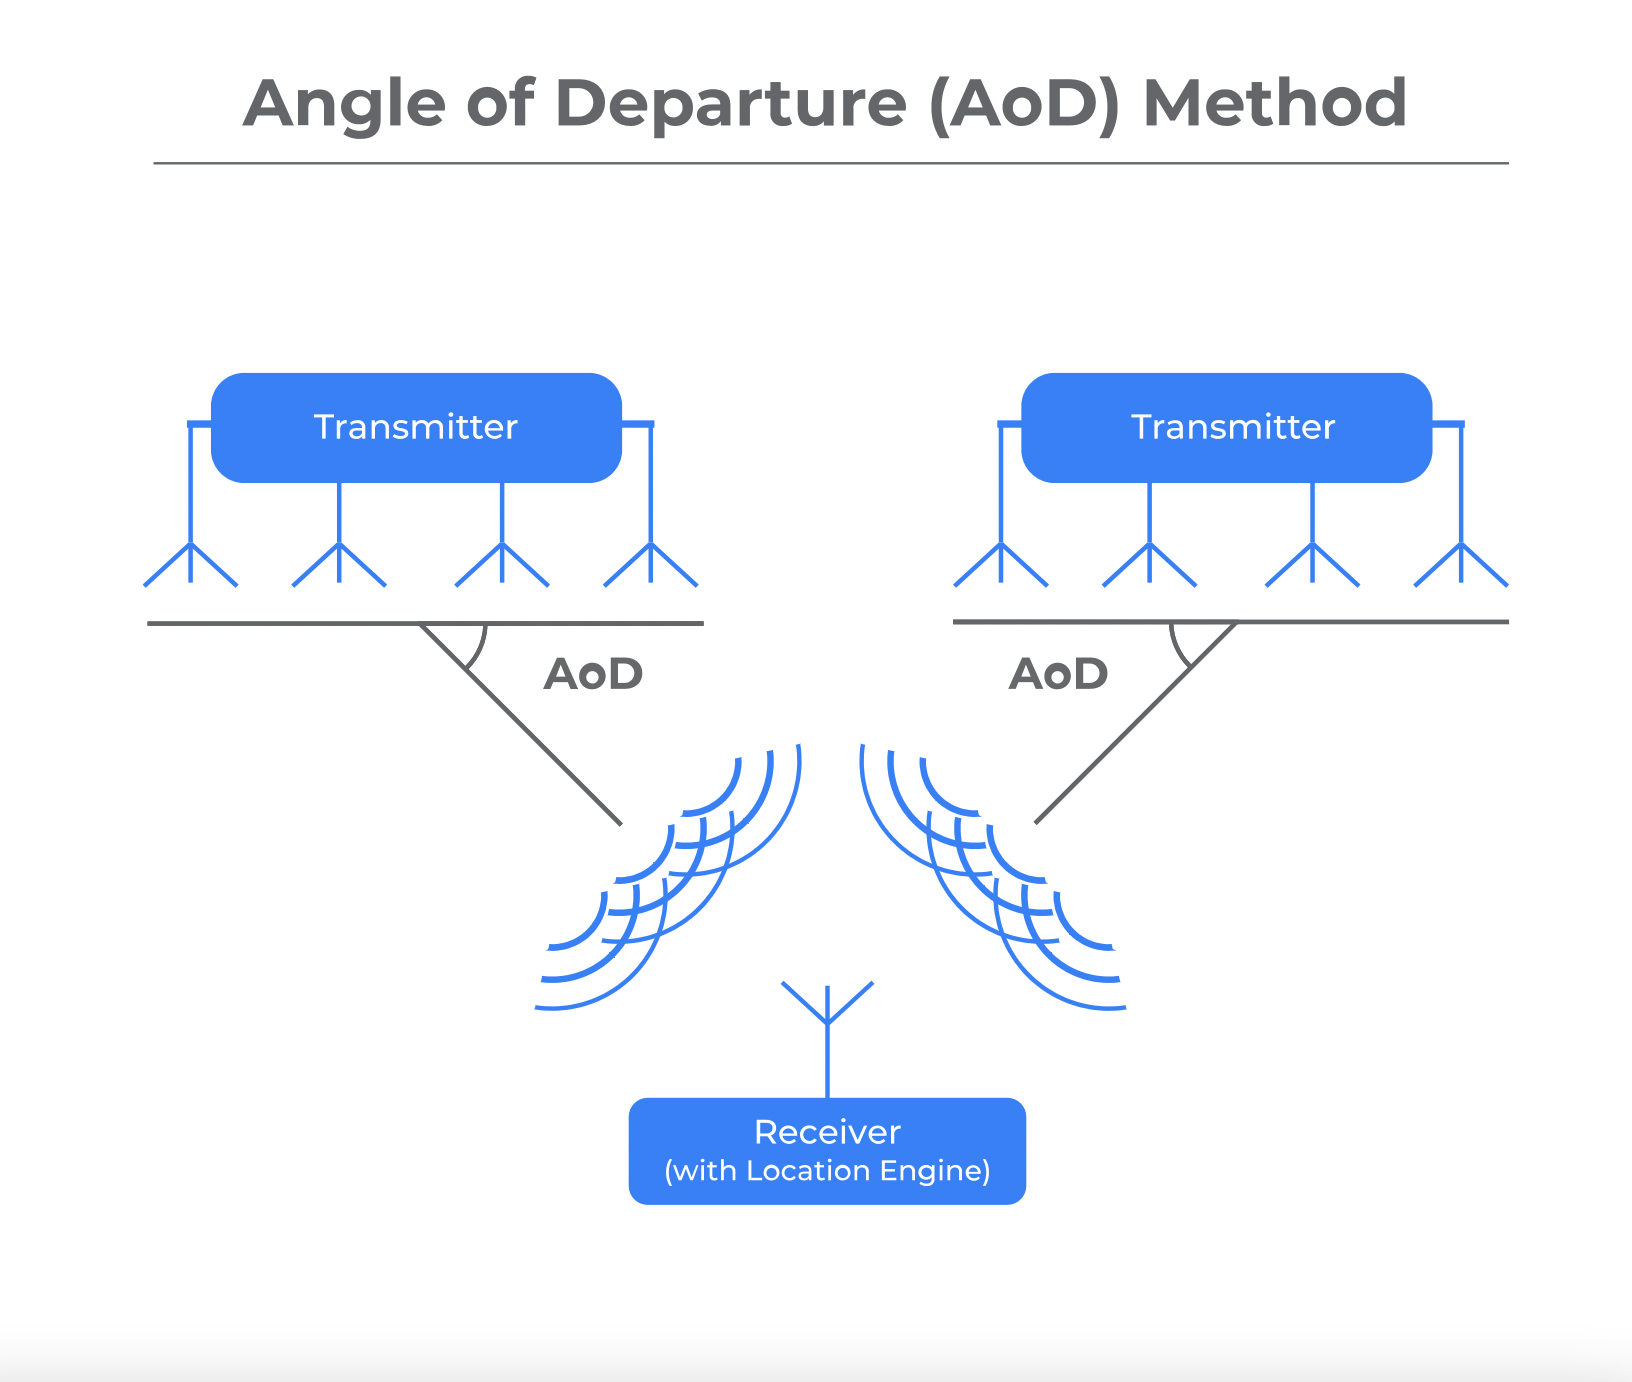
\includegraphics[width=\linewidth]{angle_of_departure_graphic.png}
%    \caption{Angle of Departure}
%    \label{fig:aop}
%\end{figure}

\subsubsection{Received Signal Strength Indicator}

De Received Signal Strength Indicator (RSSI)

\subsection{Smartphones}

Hoe werkt BLE bij smartphone?

Smartphones doen dit aan de hand van RSS \autocite{Chen2017}.


\subsection{Hoe veilig is Bluetooth Low Energy?}

%%=============================================================================
%% Methodologie
%%=============================================================================

\chapter{\IfLanguageName{dutch}{Methodologie}{Methodology}}%
\label{ch:methodologie}

%% TODO: Hoe ben je te werk gegaan? Verdeel je onderzoek in grote fasen, en
%% licht in elke fase toe welke stappen je gevolgd hebt. Verantwoord waarom je
%% op deze manier te werk gegaan bent. Je moet kunnen aantonen dat je de best
%% mogelijke manier toegepast hebt om een antwoord te vinden op de
%% onderzoeksvraag.

Zoals eerder vermeld zal, dit onderzoek zich focussen op het voorstel dat Bluetooth Low Energy een optimale oplossing is voor asset tracking in de bouwindustrie. Tegenwoordig worden daar vooral andere technologieën voor gebruikt. BLE zit daar reeds tussen, maar in veel mindere mate. In dit gedeelte van de scripte zal er een requirements-analyse uitgevoerd worden waarin alle functionele en niet-functionele vereisten uitgezocht zullen worden. Vervolgens zal er een long en short list opgesteld worden waarin alle technologieën, die vandaag de dag voornamelijk gebruikt worden, aan bod zullen komen, vergeleken en gefilterd zullen worden op geschiktheid. Hierin zal ook een grondige beschrijving aanwezig zijn van alle voor -en nadelen van BLE. Ook bestaat dit deel uit een toelichting van alle geschikte protocols, software en hardware. Op basis hiervan zal er een experimenteel onderzoek plaatsvinden aan de hand van een zelfontwikkelde Android-applicatie.

\subsection{Requirements-analyse}
Om een correcte vergelijking te maken tussen de meest frequent voorkomende technologieën die gebruikt worden om zaken als machines, voertuigen, werkmateriaal of personeel te traceren op een bouwwerf moet er enkele functionele en niet-functionele vereisten opgelijst worden. Deze zullen de beslissingsfactoren zijn waarom een bepaalde technologie boven een ander wordt verkozen. Aan de hand van deze factoren zal de hierna opgelijste long list geoptimaliseerd worden naar een short list waarin enkel de beste kandidaten nog aanwezig zijn.\\

Voor functionele vereisten gaan we kijken naar zaken die definiëren wat het systeem moet doen om aan de behoeften en verwachtingen van de gebruiker te voldoen. Zaken die hier onder ressorteren zijn bijvoorbeeld het kunnen traceren van een bepaald activa binnen een bepaalde voorafbepaalde radius en een liefst zo klein mogelijke foutmarge hebben tussen de locatie in werkelijkheid en degene aangegeven op de gebruikte software. Dit laatste, ook wel traceernauwkeurigheid genoemd, is een interessant gegeven om te vergelijken aangezien bepaalde technologieën bekend staan om een accuratere plaatsbepaling te hebben dan andere.\\

Voor niet-functionele vereisten gaan we kijken naar zaken die de werking van een systeem kunnen beoordelen, in plaats van specifiek gedrag. Deze eisen staan tegenover de functionele eisen, die hierboven beschreven staan, die specifiek gedrag of functies definiëren. Vereisten die hier ressorteren zijn zaken als initiële en operationele kosten, beveiliging, installatiegemak en het onderhoud van hardware.

\subsection{Long list}
De meest frequent voorkomende technologieën om activa te traceren op een bouwwerf zijn in de literatuurstudie van deze scriptie reeds opgelijst en beschreven geweest. In dit gedeelte van de scriptie zullen deze technologieën met elkaar vergeleken worden aan de hand van functionele en niet-functionele vereisten die in de rubriek hierboven vastgesteld zijn geweest.\\

De zes reeds beschreven technologieën zijn Global Positioning System (GPS), Radio Frequentie Identifier(RFID), Ultra-wideband (UWB), Barcode, QR Codes en Bluetooth Low Energy (BLE). Deze technologieën zullen met elkaar vergeleken worden door middel van volgende functionele en niet-functionele criteria:

\begin{itemize}
    \item Dekking
    \item Traceernauwkeurigheid
    \item Kosten
    \item Beveiliging
    \item Installatiegemak
    \item Onderhoud
\end{itemize}

Uit deze vergelijking zal een kleinere lijst gevormd worden (short list) met de technologieën die het meest potentieel hebben. Deze zullen dan meer in detail bekeken en vergeleken worden welke van de vijf technologieën het meest geschikt is voor de use-case die deze scriptie behandeld namelijk asset tracking op een bouwwerf. Hieruit zal een tijdelijke conclusie opgebouwd worden.\\

\begin{table}
\tiny
\begin{tabularx}{\textwidth} { 
        | >{\raggedright\arraybackslash}X 
        | >{\centering\arraybackslash}X 
        | >{\centering\arraybackslash}X 
        | >{\centering\arraybackslash}X 
        | >{\centering\arraybackslash}X 
        | >{\centering\arraybackslash}X 
        | >{\centering\arraybackslash}X 
        | >{\centering\arraybackslash}X | }
\hline
 & GPS & RFID & UWB & Barcode & QR Codes & BLE \\
\hline
Werkgebied & $\infty$ & <100m & <200m & Nvt & Nvt & < 100m\\
Nauwkeurigheid & <10m & <10cm & <30cm & Nvt & Nvt & 2-3m \\
Beveiliging & \\
Installatiekosten & Goedkoop & Duur & Goedkoop & Goedkoop & Goedkoop & Goedkoop \\
Onderhoudskosten & Duur & Goedkoop & Goedkoop & Goedkoop & Goedkoop & Goedkoop  \\
Tag prijs & \euro25 tot \euro50 & 50 cent tot \euro100 & >\euro100 & Afhankelijk & Gratis - afhankelijk & \euro5 tot \euro100 \\
Functie & Identificatie en lokalisatie & Identificatie & Identificatie en lokalisatie & Identificatie & Identificatie & Identificatie en lokalisatie \\
\hline
\end{tabularx}
\caption{Een vergelijking van alle mogelijke asset tracking technologieën volgens bepaalde criteria. De meeste data voor deze tabel werd uit een eerder uitgevoerde studie overgenomen, geschreven door \textcite{Ahmed2020}.}
\label{tab:technologies}
\end{table}

Uit tabel \ref{tab:technologies} kunnen verschillende dingen gelezen en afgeleid worden. Uit deze oppervlakkige verschillen kan al snel een conclusie gemaakt worden welke technologieën meer geschikt zijn dan anderen, hieruit ontstaat dan een specifiekere lijst met kandidaten volgens geschiktheid. \\

Het eerste criteria is werkgebied. Dit toont de afstand waarop een tag bereikt kan worden. Als gekeken wordt naar de verschillende technologieën zijn er meteen zaken die opvallen. Beginnend bij GPS waarbij kan geobserveerd worden dat het werkbereik oneindig is. Dit betekend dat een GPS tag van overal ter wereld bereikt kan worden. Dit is logisch aangezien een GPS tag een simkaart bevat die de positionele en soms ook andere data doorstuurt naar de servers van de gekozen provider over het mobiel netwerk, zoals reeds uitgelegd is geweest. Wat voor dit criteria nog opvalt is dat er bij barcode en QR code 'niet van toepassing' bijstaat. Vanzelfsprekend aangezien barcode en QR code functioneel niet geschikt zijn voor lokalisatie. Barcodes en QR codes kunnen wel van op een afstand gescand worden, maar dit is enkel mogelijk indien er een directe gezichtslijn is met de barcode of QR code. De afstand wordt uiteindelijk bepaald door de resolutie van de barcode of QR code. Als gekeken wordt naar de overige technologieën kan geobserveerd worden dat RFID en BLE gelijk staan en dat UWB het grootste werkgebied heeft. Deze waarden zijn zeker niet vast en kunnen veel afwijken. Dit is data verzameld door \textcite{Roberts2006} en wijkt voor RFID soms honderden meters af van andere data op het internet. Het werkgebied van technologieën als RFID, UWB of BLE hangt dus volledig af van het soort tag. 

RFID heeft twee soorten tags, namelijk actief en passieve tags. Actieve tags hebben een externe energiebron, meestal een batterij. Dit betekent dat actieve tags van veel verder gelezen kunnen worden. Passieve tags halen hun vermogen uit de transmissie van de lezer via inductieve koppeling \autocite{Roberts2006}. De passieve tags reageren dan op dat signaal. Inductieve koppeling vereist gewoonlijk dat het signaal van redelijk dichtbij verstuurd wordt. Actieve tags langs de andere kant communiceren gewoonlijk via propagatiekoppeling en reageren op de transmissie van de lezer door gebruik te maken van intern vermogen, zoals eerder vermeld.

Net zoals bij RFID is het werkgebied van UWB en BLE tags volledig afhankelijk van het soort tag dat gebruikt wordt. In het geval van BLE en UWB wordt het werkbereik bepaald door de combinatie van chipset, antenne en pad verlies. Pad verlies is de maat waarin vermogen van een radiosignaal uitgedrukt wordt dat verloren gaat onderweg van de zender tot de ontvanger \autocite{Tosi2017}. Het wordt gedefinieerd als het verschil tussen het vermogen van de zender en de gevoeligheid van de ontvanger, beiden uitgedrukt in dBm (decibel-milliwatts). Het verband tussen pad verlies en afstand (d) wordt in figuur \ref{fig:range} weergegeven. De vergelijking is wel alleen maar geldig voor een isotrope antenne en houdt geen rekening met eventuele verliezen, reflectie, ruis of obstakels in de omgeving. Het werkgebied kan door deze factoren drastisch variëren. Dit geld natuurlijk voor alle technologieën waar radio frequentie aan te pas komt.\\ 

\begin{figure}
    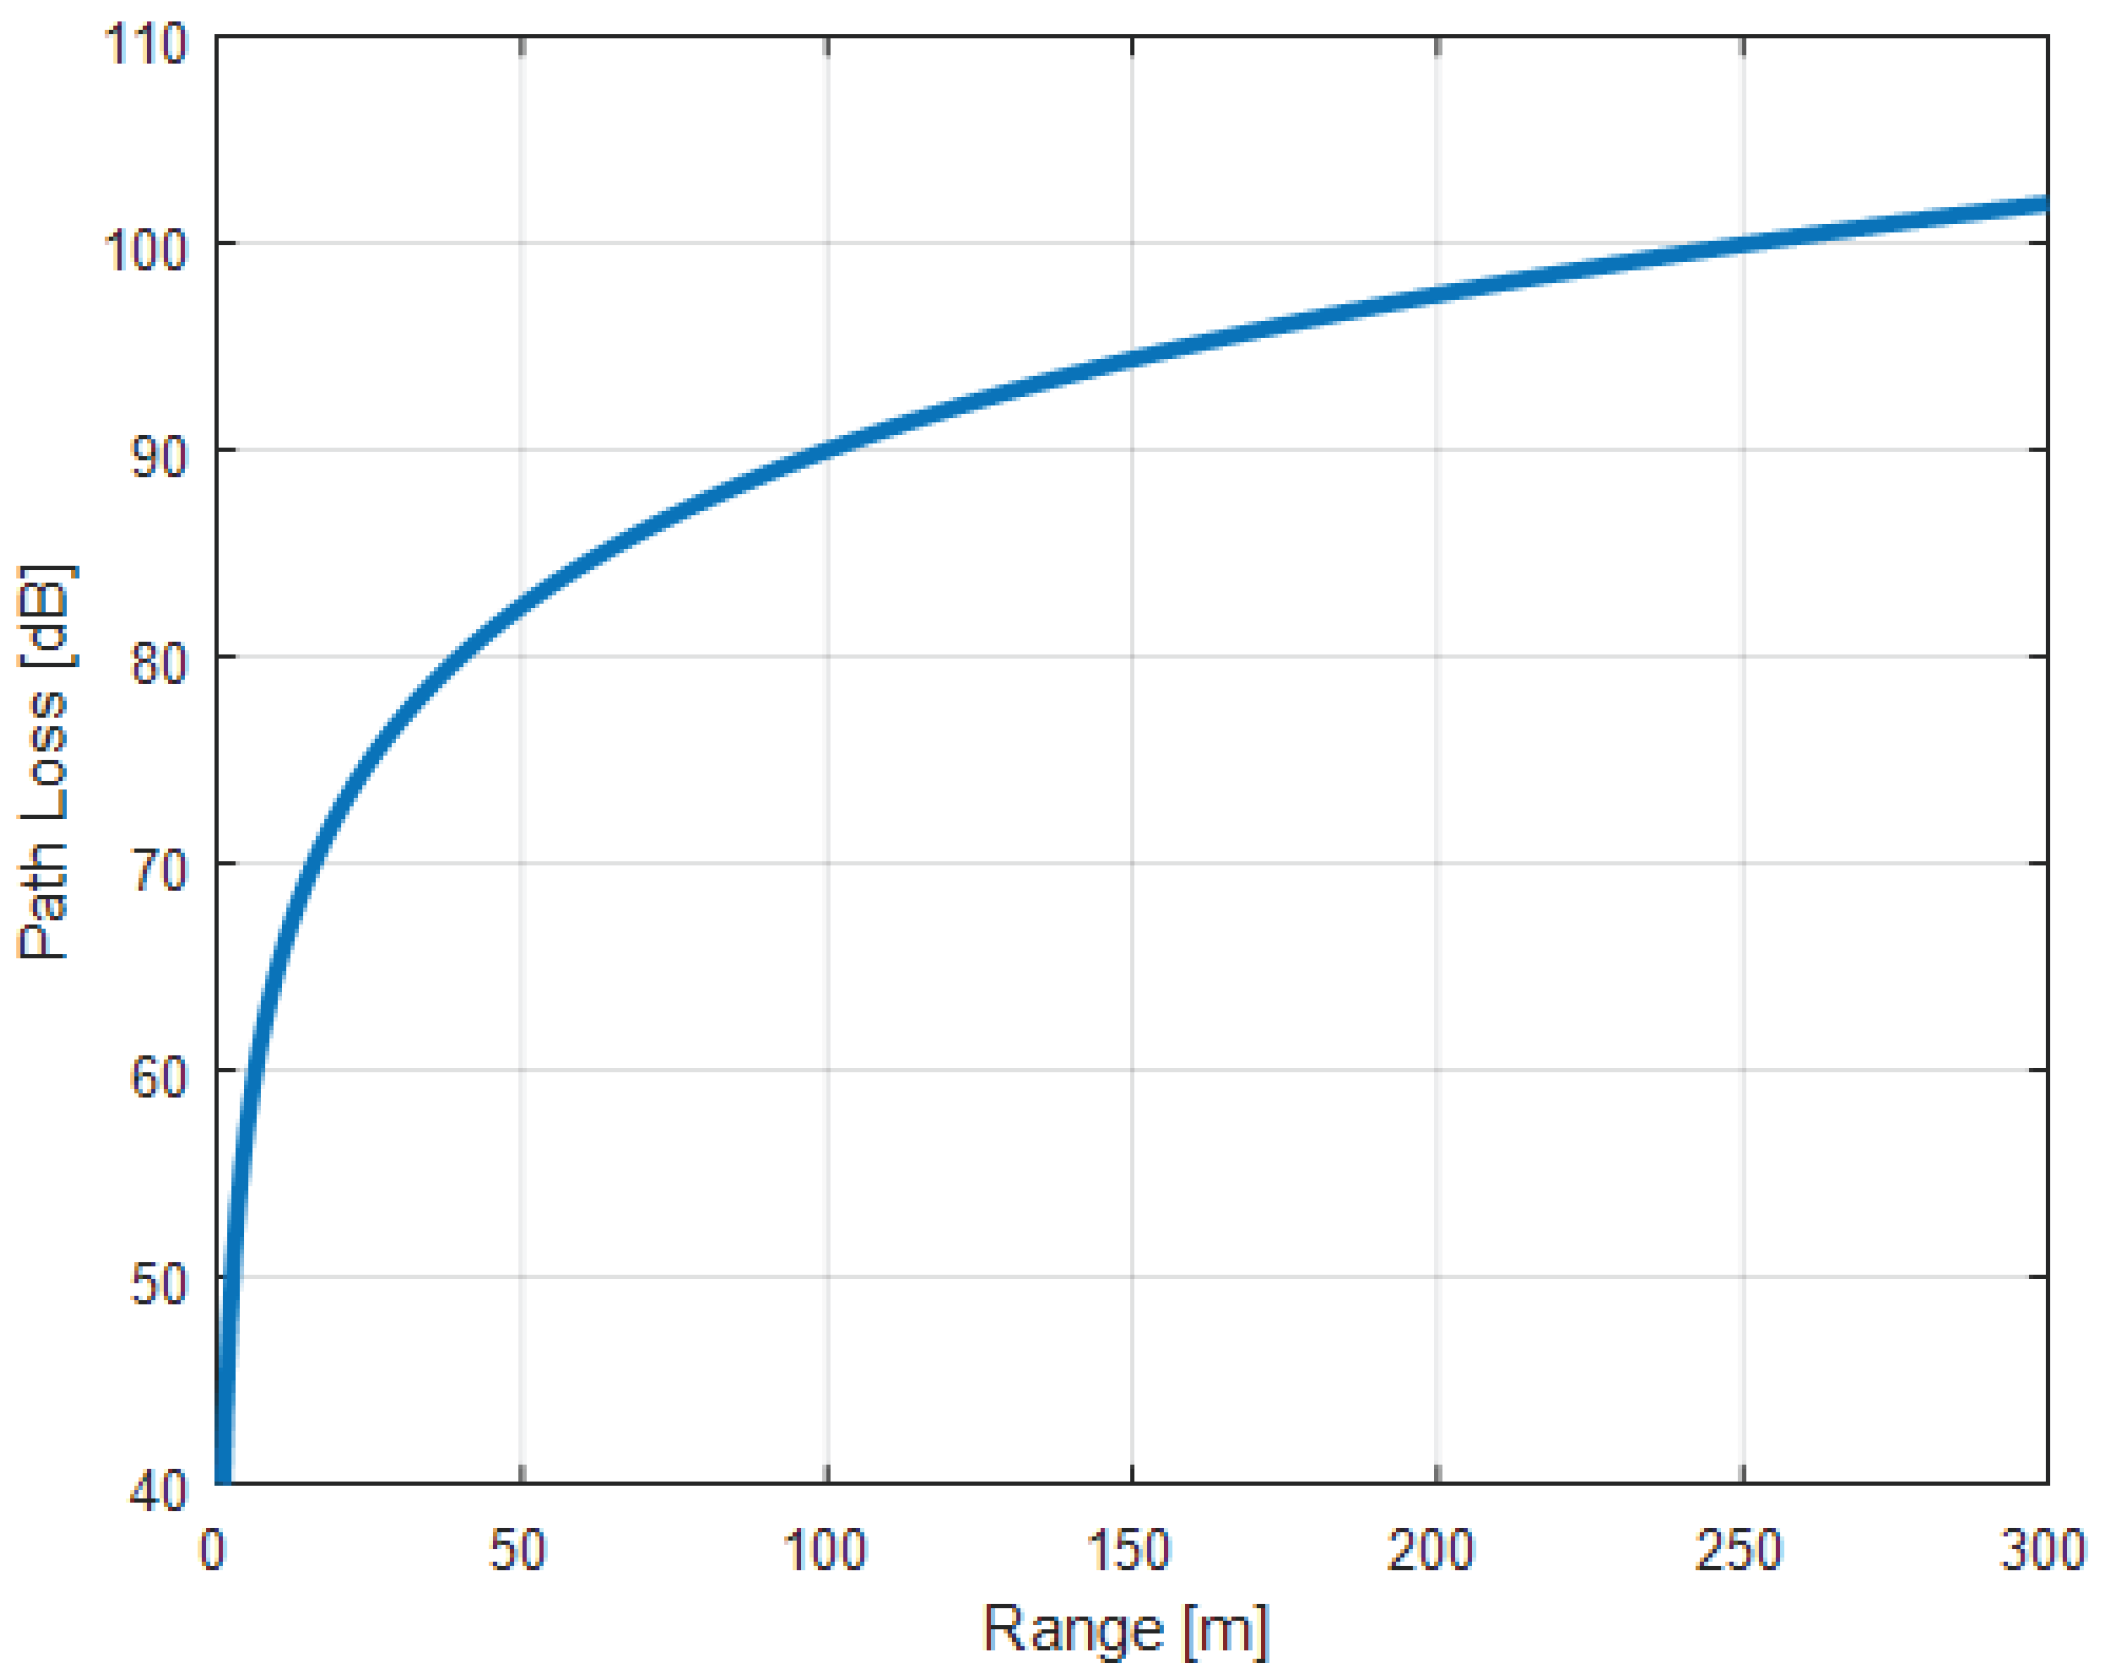
\includegraphics[\textwidth]{range.png}
    \caption[Barcode]{Een grafische representatie van pad verlies, verkregen door vergelijking \ref{pathloss} uit \autocite{Tosi2017}}
    \label{fig:range}
\end{figure}

\begin{equation}
    \label{pathloss}
    pathloss=40+25×log(d)
\end{equation}
\\

Onderhoudskosten - beter dan dit kan natuurlijk niet, maar dit komt met een prijskaartje

De laatste criteria is de functie van de technologieën. Aan de hand van dit criteria kan makkelijk bepaald worden wat de mogelijkheden zijn van een bepaalde technologie. Iedere technologie blijkt de mogelijkheid tot identificatie te hebben maar wat voor dit vergelijkend onderzoek belangrijk is, is of de technologie mogelijkheid biedt tot lokalisatie. Als we de technologieën overlopen zien we meteen twee technologieën die eruit springen. Dit zijn barcode en QR code. Bij deze twee is het niet mogelijk om op een of andere manier de locatie van het activa waaraan de code bevestigd is te lokaliseren. Voor de onderzoeksvraag van deze scriptie is het wel van cruciaal belang dat dit mogelijk is en daarom zullen we deze twee technologieën achterwegen laten voor deze vergelijkende studie.\\

Het tweede criteria is traceernauwkeurigheid. Indien een bouwwerf van kleine oppervlakte is of de te traceren activa dicht bij elkaar staan is het van belang dat deze makkelijk gelokaliseerd kan worden en dat deze activa niet met elkaar verwisseld worden door een slechte traceernauwkeurigheid. Aangezien barcode en QR code niet van op afstand traceerbaar zijn zullen deze vanzelfsprekend niet meegerekend worden. De traceernauwkeurigheid bij deze twee technologieën zal altijd 100\% zijn aangezien de activa eerst handmatig gelokaliseerd moet worden voor de code gescand kan worden.

De waarden van de andere technologieën zijn vrij verschillend. De technologie die er een beetje uitsteekt is GPS. Dit is geweten dat GPS in het algemeen het minst exact de locatie van iets weergeeft. De afstand kan variëren van een paar meter tot precies. Zo een afwijking kan veroorzaakt worden door verschillende zaken zoals satellietgeometrie, signaal obstructie of atmosferische omstandigheden.

Bij de andere technologieën is er nog maar een technologie dat meer dan een meter afwijkt en dit is BLE. Om de afstand te bepalen tussen een zendende (TX) en een ontvangende (RX) node wordt bij BLE Received Signal Strength Indicator (RSSI) gebruikt. Dit is de reden voor de afwijking bij de traceernauwkeurigheid van BLE. RSSI wordt berekend aan de hand van vergelijking \ref{rssi}.

\begin{equation}
    \label{rssi}
    RSSI=−10×N×log(d)+a
\end{equation}

Hierin is $N$ een constante die als één wordt aangenomen, $d$ de afstand in meters tussen de twee apparaten en $a$ het vermogen van de TX op één meter afstand.

\subsection{Short list}
Twee technologieën zijn duidelijk niet geschikt voor asset tracking op een bouwwerf, namelijk barcode en QR code. De reden hiervoor is dat activa waarop een code bevestigd is niet van op afstand gelokaliseerd kan worden. Dit is van cruciaal belang indien men snel activa wil lokaliseren in een complexe en drukke omgeving als een bouwwerf. Indien de overgebleven technologieën nog eens naast elkaar gelegd worden komen we bij tabel \ref{tab:technologies2} uit. Hier zijn er wat extra criteria bijgevoegd aangezien de technologieën op specifiekere vlakken met elkaar verschillen die in de praktijk minstens even belangrijk zouden kunnen zijn om de meest geschikte technologie voor asset tracking op een bouwwerf te kiezen. Dit zijn zaken zoals de levensduur van batterijen, energieverbruik en of de technologie compatibel is met smartphones. 

\begin{table}
    \tiny
    \begin{tabularx}{\textwidth} { 
            | >{\raggedright\arraybackslash}X 
            | >{\centering\arraybackslash}X 
            | >{\centering\arraybackslash}X 
            | >{\centering\arraybackslash}X 
            | >{\centering\arraybackslash}X 
            | >{\centering\arraybackslash}X 
            | >{\centering\arraybackslash}X 
            | >{\centering\arraybackslash}X | }
        \hline
        & GPS & RFID & UWB & BLE \\
        \hline
        Functie & Identificatie en lokalisatie & Identificatie & Identificatie en lokalisatie & Identificatie en lokalisatie \\
        Werkgebied & $\infty$ & <100m & <200m & < 100m\\
        Nauwkeurigheid & <10m & <10cm & <30cm & 2-3m \\
        Beveiliging & \\
        Installatiekosten & Goedkoop & Duur & Goedkoop & Goedkoop \\
        Onderhoudskosten & Duur & Goedkoop & Goedkoop & Goedkoop  \\
        Tag prijs & \euro25 tot \euro50 & 50 cent tot \euro100 & >\euro100 & \euro5 tot \euro100 \\
        \hline
        Batterij & <3 jaar & 3-5 jaar & <2 jaar & 2-5 jaar \\
        Energieverbruik & Laag & Laag/Hoog & Laag & Laagst\\
        Smartphone compatibiliteit & $\bullet$ & & $\bullet$ & $\bullet$ \\
        \hline
    \end{tabularx}
    \caption{Een nauwkeurigere vergelijking van verschillende geschikte asset tracking technologieën volgens bepaalde criteria. De data voor deze tabel werd net zoals bij tabel \ref{tab:technologies} uit een eerder uitgevoerde studie overgenomen, geschreven door \textcite{Ahmed2020}.}
    \label{tab:technologies2}
\end{table}

smartphone compatibliteit rfid https://gadgetfaculty.com/smartphone-rfid-reader-rfid-tag/
uhf is not compatible with nfc

\subsection{Conclusie vergelijkende studie}
Hier zal een conclusie opgesteld worden aan de hand van de vergelijkende studie die uitgevoerd is geweest in de rubriek hierboven. Deze conclusie, samen met de uitkomst van de proof of concept zullen dan de eindconclusie bepalen.

%TODO:Vergelijking tussen de verschillende techologien, tabel maken en alles volluit uitgeschreven uitgelegd erbij

%TODO: De eerste fase is een introductie over de pro-blematiek. Dit wordt gerealiseerd door een gron-dige studie van vakliteratuur, zoals wetenschap-pelijke teksten of blogs. Hieruit volgt een tekstdie alle vereisten aanhaalt voor een optimale op-lossing. De geschatte duurtijd van deze fase be-draagt twee weken.
\subsection{Voordelen van BLE asset tracking}
Hier zullen alle voordelen van BLE asset tracking beschreven worden en nog een vergeleken worden met andere technologieën.
%TODO: De tweede fase houdt een analyse in van wetenschappelijke teksten, met als resultaat een uitgebreide tekst over de voordelen van BLE asset tracking, ten opzichte van technologieën die van-daag de dag gebruikt worden. Hiervoor is een week genoeg.
\subsection{Nadelen van BLE asset tracking}
Hier zullen alle nadelen van BLE asset tracking beschreven worden en nog een vergeleken worden met andere technologieën.
%TODO: De derde fase is opnieuw een beschrijving,maar dan over de valkuilen van BLE asset tracking.  Deze fase van het onderzoek brengt alle mogelijke tekortkomingen in kaart.  Ook voor deze fase is een week voldoende.
\subsection{Toelichting van protocols, hardware en software}
In dit gedeelte zal een toelichting van alle bestaande protocols van beacons en tags beschreven worden. Hierbij wordt er gezocht naar de meest geschikte hardware waarbij er nauwkeurig afgewogen moet worden tussen kosten en functionaliteit. 
%TODO: De vierde fase bestaat uit het toelichten van de meest geschikte protocols, compatibiliteit van software en hardware ,zoals beacons en gateways.Hierbij wordt er gezocht naar de meest geschikte hardware waarbij er nauwkeurig afgewogen moet worden tussen kosten en functionaliteit. Vervolgens wordt er een veldonderzoek uitgevoerd om,naargelang de vereisten, de keuze te maken op welke manier de app ontwikkeld zal worden. Tot slot zullen alle beschikbare protocols in kaart gebracht worden. De geschatte duurtijd van deze fase bedraagt drie weken.
\subsection{Proof of Concept}



% Voeg hier je eigen hoofdstukken toe die de ``corpus'' van je bachelorproef
% vormen. De structuur en titels hangen af van je eigen onderzoek. Je kan bv.
% elke fase in je onderzoek in een apart hoofdstuk bespreken.

%\input{...}
%\input{...}
%...

%%=============================================================================
%% Conclusie
%%=============================================================================

\chapter{Conclusie}%
\label{ch:conclusie}

% TODO: Trek een duidelijke conclusie, in de vorm van een antwoord op de
% onderzoeksvra(a)g(en). Wat was jouw bijdrage aan het onderzoeksdomein en
% hoe biedt dit meerwaarde aan het vakgebied/doelgroep? 
% Reflecteer kritisch over het resultaat. In Engelse teksten wordt deze sectie
% ``Discussion'' genoemd. Had je deze uitkomst verwacht? Zijn er zaken die nog
% niet duidelijk zijn?
% Heeft het onderzoek geleid tot nieuwe vragen die uitnodigen tot verder 
%onderzoek?




%---------- Bijlagen -----------------------------------------------------------

\appendix

\chapter{Onderzoeksvoorstel}

Het onderwerp van deze bachelorproef is gebaseerd op een onderzoeksvoorstel dat vooraf werd beoordeeld door de promotor. Dat voorstel is opgenomen in deze bijlage.

%% TODO: 
%\section*{Samenvatting}

% Kopieer en plak hier de samenvatting (abstract) van je onderzoeksvoorstel.

% Verwijzing naar het bestand met de inhoud van het onderzoeksvoorstel
%---------- Inleiding ---------------------------------------------------------

\section{Introductie}%
\label{sec:introductie}



Bluetooth Low Energy (BLE) is een eenvoudige draadloze netwerktechnologie \autocite{Heydon2013}, onafhankelijk van het klassieke Bluetooth. Het is geoptimaliseerd voor ultra laag energieverbruik en een lagere datacapaciteit. BLE wordt standaard ondersteund door zo goed als alle populaire operating systems zoals iOS, Android, macOS en Windows.

Een technologie zoals deze kan gebruikt worden in diverse sectoren met verschillende toepassingen. Enkele van deze toepassingen zijn bijvoorbeeld access control, blood monitoring en smart watches, maar in deze scriptie zal er gefocust worden op asset tracking op een bouwwerf. Hierrond kunnen verschillende vraagstellingen geformuleerd worden.

In dit onderzoek wordt een proof of concept uitgevoerd om de huidige manier van asset tracking op een bouwwerf te optimaliseren aan de hand van BLE beacons, BLE tags, gateways en compatibele smartphones.
Er zal ook een algemene analyse gebeuren van de beveiliging van BLE. Hoewel de beveiligingsfuncties in de loop der jaren opmerkelijk zijn verbeterd, is de BLE-technologie nog steeds vatbaar voor ernstige bedreigingen \autocite{Lacava_2022}, waardoor een kloof ontstaat tussen het theoretische standaardontwerp en de uitvoering ervan.

Het doel van dit onderzoek is om een introductie te geven tot de problematiek en waarom dit een verbetering zou kunnen zijn op de huidige manier van asset tracking. Vervolgens volgt er een analyse van wetenschappelijke teksten en artikels, waaruit alle voordelen en nadelen van het gebruik van BLE, in de context van asset tracking, op een bouwwerf voorkomen. Daaropvolgend wordt er op zoek gegaan naar de meest geschikte protocols, compatibiliteit van software en hardware zoals beacons en gateways. Tot slot wordt een app samengesteld waarmee assets gelokaliseerd en gevisualiseerd kunnen worden, waarna advies over de meest optimale oplossing verleend wordt.

%Waarover zal je bachelorproef gaan? Introduceer het thema en zorg dat volgende zaken zeker duidelijk aanwezig zijn:

%\begin{itemize}
%  \item kaderen thema
%  \item de doelgroep
%  \item de probleemstelling en (centrale) onderzoeksvraag
%  \item de onderzoeksdoelstelling
%\end{itemize}
%
%Denk er aan: een typische bachelorproef is \textit{toegepast onderzoek}, wat betekent dat je start vanuit een concrete probleemsituatie in bedrijfscontext, een \textbf{casus}. Het is belangrijk om je onderwerp goed af te bakenen: je gaat voor die \textit{ene specifieke probleemsituatie} op zoek naar een goede oplossing, op basis van de huidige kennis in het vakgebied.
%
%De doelgroep moet ook concreet en duidelijk zijn, dus geen algemene of vaag gedefinieerde groepen zoals \emph{bedrijven}, \emph{developers}, \emph{Vlamingen}, enz. Je richt je in elk geval op it-professionals, een bachelorproef is geen populariserende tekst. Eén specifiek bedrijf (die te maken hebben met een concrete probleemsituatie) is dus beter dan \emph{bedrijven} in het algemeen.
%
%Formuleer duidelijk de onderzoeksvraag! De begeleiders lezen nog steeds te veel voorstellen waarin we geen onderzoeksvraag terugvinden.
%
%Schrijf ook iets over de doelstelling. Wat zie je als het concrete eindresultaat van je onderzoek, naast de uitgeschreven scriptie? Is het een proof-of-concept, een rapport met aanbevelingen, \ldots Met welk eindresultaat kan je je bachelorproef als een succes beschouwen?

%---------- Stand van zaken ---------------------------------------------------

\section{State-of-the-art}%
\label{sec:state-of-the-art}

Op een bouwwerf worden vandaag de dag heel wat traceertechnologieën gebruikt \autocite{Nasr2013}, aangezien deze hebben aangetoond efficiënt en betaalbaar te zijn. Enkele hiervan zijn Ultra-Wide Bands (UWB), Radio Frequency Identification Cards (RFID) en Global Positioning Systems (GPS). Real-time assets zoals werkmateriaal, machines en werkpersoneel kunnen aan de hand hiervan getraceerd worden. 

Een Bluetooth Low Energy  beacon of tag is een simpel toestel dat niet meer hoeft te zijn dan een CPU, radio en batterij. Het is een radio transmitter \autocite{Andony2022} die BLE signalen verstuurt zodat die geïnterpreteerd kunnen worden door compatibele apps of operating systems binnen een bepaalde afstand. Dit signaal is meestal een uniek ID nummer. Door dit signaal kan ook de locatie van de beacon of tag bepaald worden door de ontvanger. Hier speelt RSSI \autocite{Subhan_2019} een belangrijke rol. Als gevolg van ruis treden er fluctuaties op in de RSSI, wat leidt tot een fout in de afstandsbepaling, die uiteindelijk invloed nauwkeurigheid van de positiebepaling beïnvloed. BLE tags kunnen bijna op elk voorwerp worden aangebracht, zodat het via Bluetooth kan worden geïdentificeerd en gevolgd. Door het minimale stroomverbruik kunnen deze bovendien langer aanstaan zonder te moeten worden opgeladen. Dit maakt BLE tags ideaal voor het volgen van inventaris of het bewaken van de locatie van waardevolle voorwerpen.

Een mogelijke vraag die kan worden gesteld is waarom BLE nog niet gebruikt wordt voor asset tracking op een bouwwerf en dat is wat in deze scriptie onderzocht wordt.

%Hier beschrijf je de \emph{state-of-the-art} rondom je gekozen onderzoeksdomein, d.w.z.\ een inleidende, doorlopende tekst over het onderzoeksdomein van je bachelorproef. Je steunt daarbij heel sterk op de professionele \emph{vakliteratuur}, en niet zozeer op populariserende teksten voor een breed publiek. Wat is de huidige stand van zaken in dit domein, en wat zijn nog eventuele open vragen (die misschien de aanleiding waren tot je onderzoeksvraag!)?
%
%Je mag de titel van deze sectie ook aanpassen (literatuurstudie, stand van zaken, enz.). Zijn er al gelijkaardige onderzoeken gevoerd? Wat concluderen ze? Wat is het verschil met jouw onderzoek?
%
%Verwijs bij elke introductie van een term of bewering over het domein naar de vakliteratuur, bijvoorbeeld~\autocite{Hykes2013}! Denk zeker goed na welke werken je refereert en waarom.
%
%Draag zorg voor correcte literatuurverwijzingen! Een bronvermelding hoort thuis \emph{binnen} de zin waar je je op die bron baseert, dus niet er buiten! Maak meteen een verwijzing als je gebruik maakt van een bron. Doe dit dus \emph{niet} aan het einde van een lange paragraaf. Baseer nooit teveel aansluitende tekst op eenzelfde bron.
%
%Als je informatie over bronnen verzamelt in JabRef, zorg er dan voor dat alle nodige info aanwezig is om de bron terug te vinden (zoals uitvoerig besproken in de lessen Research Methods).

% Voor literatuurverwijzingen zijn er twee belangrijke commando's:
% \autocite{KEY} => (Auteur, jaartal) Gebruik dit als de naam van de auteur
%   geen onderdeel is van de zin.
% \textcite{KEY} => Auteur (jaartal)  Gebruik dit als de auteursnaam wel een
%   functie heeft in de zin (bv. ``Uit onderzoek door Doll & Hill (1954) bleek
%   ...'')

%Je mag deze sectie nog verder onderverdelen in subsecties als dit de structuur van de tekst kan verduidelijken.

%---------- Methodologie ------------------------------------------------------
\section{Methodologie}%
\label{sec:methodologie}

Het onderzoek houdt zes fasen in. In deze fasen wordt er een kleine vergelijkende studie uitgevoerd en een Proof of Concept opgesteld.

De eerste fase is een introductie over de problematiek. Dit wordt gerealiseerd door een grondige studie van vakliteratuur, zoals wetenschappelijke teksten of blogs. Hieruit volgt een tekst die alle vereisten aanhaalt voor een optimale oplossing. De geschatte duurtijd van deze fase bedraagt twee weken.

De tweede fase houdt een analyse in van wetenschappelijke teksten, met als resultaat een uitgebreide tekst over de voordelen van BLE asset tracking, ten opzichte van technologieën die vandaag de dag gebruikt worden. Hiervoor is een week genoeg.

De derde fase is opnieuw een beschrijving, maar dan over de valkuilen van BLE asset tracking. Deze fase van het onderzoek brengt alle mogelijke tekortkomingen in kaart. Ook voor deze fase is een week voldoende.

De vierde fase bestaat uit het toelichten van de meest geschikte protocols, compatibiliteit van software en hardware ,zoals beacons en gateways. Hierbij wordt er gezocht naar de meest geschikte hardware waarbij er nauwkeurig afgewogen moet worden tussen kosten en functionaliteit. Vervolgens wordt er een veldonderzoek uitgevoerd om, naargelang de vereisten, de keuze te maken op welke manier de app ontwikkeld zal worden. Tot slot zullen alle beschikbare protocols in kaart gebracht worden. De geschatte duurtijd van deze fase bedraagt drie weken.

De vijfde fase van dit onderzoek bedraagt het ontwikkelen van een applicatie waarmee assets gelokaliseerd en gevisualiseerd kunnen worden. Deze app wordt verwacht in .NET te worden geschreven voor het Android operating system. De geschatte duurtijd van deze fase bedraagt vier weken.

De zesde en laatste fase bevat een verduidelijking van de bekomen resultaten, met als doel te bewijzen dat het voorgestelde concept, asset tracking a.d.h.v. Bluetooth Low Energy, een optimale manier is. De geschatte duurtijd van deze fase bedraagt een week.


%Hier beschrijf je hoe je van plan bent het onderzoek te voeren. Welke onderzoekstechniek ga je toepassen om elk van je onderzoeksvragen te beantwoorden? Gebruik je hiervoor literatuurstudie, interviews met belanghebbenden (bv.~voor requirements-analyse), experimenten, simulaties, vergelijkende studie, risico-analyse, PoC, \ldots?
%
%Valt je onderwerp onder één van de typische soorten bachelorproeven die besproken zijn in de lessen Research Methods (bv.\ vergelijkende studie of risico-analyse)? Zorg er dan ook voor dat we duidelijk de verschillende stappen terug vinden die we verwachten in dit soort onderzoek!
%
%Vermijd onderzoekstechnieken die geen objectieve, meetbare resultaten kunnen opleveren. Enquêtes, bijvoorbeeld, zijn voor een bachelorproef informatica meestal \textbf{niet geschikt}. De antwoorden zijn eerder meningen dan feiten en in de praktijk blijkt het ook bijzonder moeilijk om voldoende respondenten te vinden. Studenten die een enquête willen voeren, hebben meestal ook geen goede definitie van de populatie, waardoor ook niet kan aangetoond worden dat eventuele resultaten representatief zijn.
%
%Uit dit onderdeel moet duidelijk naar voor komen dat je bachelorproef ook technisch voldoen\-de diepgang zal bevatten. Het zou niet kloppen als een bachelorproef informatica ook door bv.\ een student marketing zou kunnen uitgevoerd worden.
%
%Je beschrijft ook al welke tools (hardware, software, diensten, \ldots) je denkt hiervoor te gebruiken of te ontwikkelen.
%
%Probeer ook een tijdschatting te maken. Hoe lang zal je met elke fase van je onderzoek bezig zijn en wat zijn de concrete \emph{deliverables} in elke fase?

%---------- Verwachte resultaten ----------------------------------------------
\section{Verwacht resultaat, conclusie}%
\label{sec:verwachte_resultaten}

Er wordt verwacht dat Bluetooth Low Energy een zeer optimale keuze is voor asset tracking binnen een bouwwerf. Met een lage kostprijs, makkelijke installatie en nauwkeurige tracering, behoort deze technologie aan de top van rendabele en duurzame mogelijkheden.

De doelgroep van dit onderzoek, namelijk werfleiders of andere leidinggevende functies kunnen op dezelfde manier hun werkmateriaal, personeel en machines traceren, maar dan veel goedkoper, accurater en mogelijks efficiënter.

%Hier beschrijf je welke resultaten je verwacht. Als je metingen en simulaties uitvoert, kan je hier al mock-ups maken van de grafieken samen met de verwachte conclusies. Benoem zeker al je assen en de onderdelen van de grafiek die je gaat gebruiken. Dit zorgt ervoor dat je concreet weet welk soort data je moet verzamelen en hoe je die moet meten.
%
%Wat heeft de doelgroep van je onderzoek aan het resultaat? Op welke manier zorgt jouw bachelorproef voor een meerwaarde?
%
%Hier beschrijf je wat je verwacht uit je onderzoek, met de motivatie waarom. Het is \textbf{niet} erg indien uit je onderzoek andere resultaten en conclusies vloeien dan dat je hier beschrijft: het is dan juist interessant om te onderzoeken waarom jouw hypothesen niet overeenkomen met de resultaten.



%%---------- Andere bijlagen --------------------------------------------------
% TODO: Voeg hier eventuele andere bijlagen toe. Bv. als je deze BP voor de
% tweede keer indient, een overzicht van de verbeteringen t.o.v. het origineel.
%\input{...}

%%---------- Backmatter, referentielijst ---------------------------------------

\backmatter{}

\setlength\bibitemsep{2pt} %% Add Some space between the bibliograpy entries
\printbibliography[heading=bibintoc]

\end{document}
